%!TEX root = ../ausarbeitung.tex
\newpage
\section{ Lokalisierung mit Principal Components Analysis (PCA)}
Die automatische Lokalisierung von Objekten in digitalen Bildern ist ein wesentlicher Bestandteil vieler Anwendungen. 
Für das Lokalisierungsproblem in dieser Arbeit bietet sich die Verwendung von der Methoden \textit{Hintergrund-Subtraktion} und \textit{Sliding-window mit PCA} an.

\subsection{Hintergrundapproximation mit PCA}
Um Bewegungen in Bildsequenzen erkennen zu können, wird in der Praxis sehr häufig das Verfahren der \textit{Hintergrund-Subtraktion} angewandt. Dabei handelt es sich um ein klassisches Verfahren aus dem Bereich der Bilderkennung. Das Hintergrundbild kann mithilfe von PCA approximiert werden. Anschließend wird das Vordergrundbild über die Differenz zum Hintergrundbild extrahiert. PCA, oder auch Haptkomponentenanalyse, ist ein statistisches Verfahren um große Mengen von Datensätzen zu vereinfachen und zu strukturieren, indem die Datenpunkte im $p$-dimensionalen Raum $R^p$ in einen $q$-dimensionalen Unterraum ${R} ^{q}$ mit ($q<p$) projiziert werden. Diese Transformation muss dabei so gewählt werden, dass möglichst wenig Information verloren geht. 
Grundsätzlich benutzt PCA die \textit{Niedrigrang Approximation}. Damit kann eine Matrix durch eine andere Matrix im allgemeinen Rang angenähert werden. Sei eine Matrix $A$ mit $Rang(A) = r$ und $r > k$:
\begin{equation}
\min_{rang(A)=k}||A-B||_2 
\end{equation}
Dabei soll die Differenz zwichen $A$ und $B$ minimiert werden. Mit Hilfe der \textit{Singulärwertzerlegung (SVD)} können die Singulärwerte einer Matrix abgelesen werden. Die SVD von Matrix $A$ ist dann:
\begin{equation}
A = U \Sigma V^T
\end{equation}
Somit kann ein Hintergrundbild aus einer Sequenz von Bildern wie folgt approximiert werden (Abbildung~\ref{fig:approx}):
\begin{itemize}
\item{Berechne Singulärwertzerlegung aller Bildern von Sequenz $X$:}
\begin{equation}
SVD(X)= C = U \Sigma V^T
\end{equation}
\item{Leite die Matrix ${\Sigma_k}$ von ${\Sigma}$ her, sodass die Werte ${n - k}$  entlang der Diagonale durch 0 ersetzt werden.}
\item{Dies ergibt die Niedrigrang Approximation vom Matrix $X$:}
\begin{equation}
SVD(X)_k=C_k = U\Sigma_kV^T \quad\quad mit  \quad  \Sigma_k = diag(\sigma_1, ..., \sigma_k,0,...,0)
\end{equation}
\end{itemize}
\newpage
\begin{center}
\begin{tabular}{ccccc}
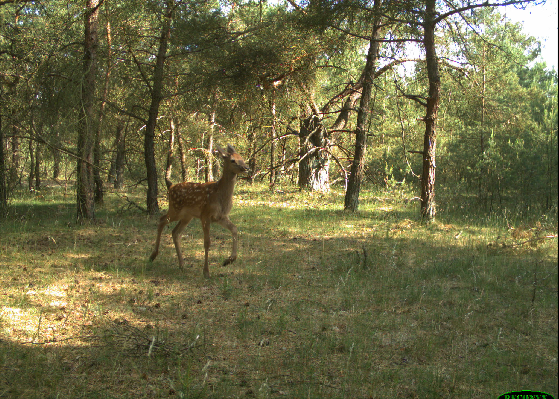
\includegraphics[width=2.3cm]{img/Segmentierung/original-image}
&
\includegraphics[width=2.3cm]{img/Segmentierung/seq2}
&
\includegraphics[width=2.3cm]{img/Segmentierung/seq4}
&
\includegraphics[width=2.3cm]{img/Segmentierung/seq3}
&
\includegraphics[width=2.3cm]{img/Segmentierung/seq5}\\
(a) & (b) &(c)&(d)&(e)
\end{tabular}
\end{center}
\begin{center}
\begin{tabular}{c}
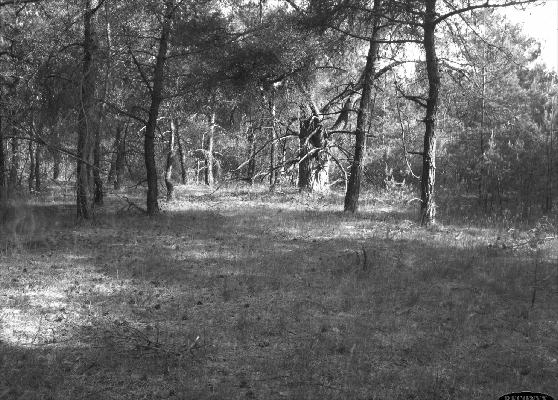
\includegraphics[width=4cm]{img/Segmentierung/background-image}\\
(f) 
\end{tabular} 
\captionof{figure}{(a)-(e) Bilder aus einer Sequenz und (f) das approximierte Hintergrundbild.}
\label{fig:approx}

\end{center}

\noindent Anschließend kann das Vordergrundbild durch die klassiche \textit{Hintergrund-Subtraktion} extrahiert werden (Abbildung~\ref{fig:foreground}).

\begin{center}
\begin{tabular}{c}
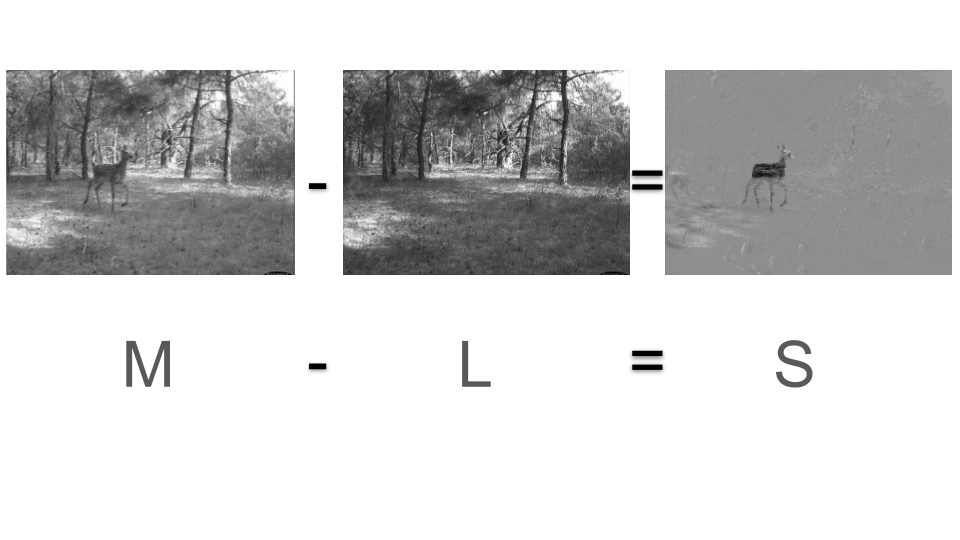
\includegraphics[width=6cm]{img/Segmentierung/foreground-image}
\end{tabular}
\captionof{figure}{Das Vordergrundbild ergibt sich durch die Subtraktion des approximierten Hintergrundbildes.}
\label{fig:foreground}
\end{center}
\noindent Zum Nachbearbeitung des Vordergrundes gehört eine Vielzahl von Operationen 
z.B. \textit{morphologische Operationen, Thresholding} und \textit{Filterung}.
Damit können kleinere Bildstrukturen und Rauschen entfernt, vergrößert, geschlossen oder aufgefüllt werden. Können jedoch diese Operationen zu einer Veränderung der Größe der Vordergrundelemente führen, was zur Lokalisierung des Elements aber keinen Störfaktor ergibt. Durch Kombination der Operationen in einer bestimmten Reihenfolge kann Größenveränderung verhindert und dennoch die Vorteile der Operationen genutzt werden. Durch \textit{Opening} werden zunächst kleine Strukturen bzw. Rauschen, welches zum Hintergrund gehört, entfernt. Danach werden kleine Löcher innerhalb der Vordergrundelemente durch \textit{Closing} geschlossen. In (Abbildung~\ref{fig:pipe}) ist eine Kombination dieser  Pipeline zur Nachbearbeitung des Vordergrundes benutzt worden.
\begin{center}
\begin{tabular}{c}
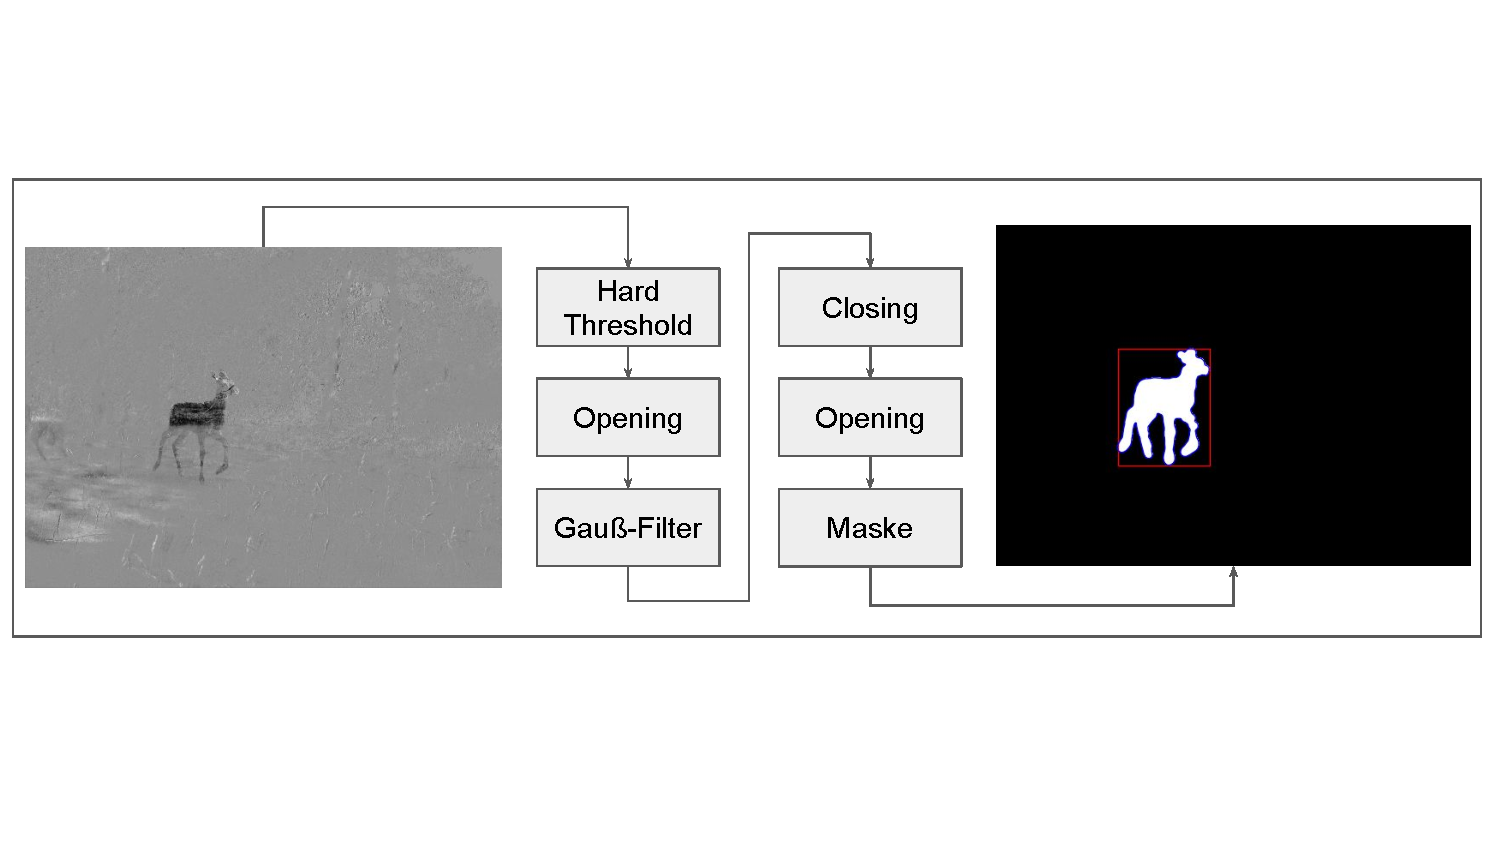
\includegraphics[trim={0 3cm 0cm 3cm},clip=true,width=13cm]{img/Segmentierung/pipe.pdf}
\end{tabular}
\captionof{figure}{Die Pipeline der Nachbearbeitung des Vordergrundbildes. Durch \textit{Opening} und \textit{Closing} werden kleine Bildstrukturen bzw. Rauschen entfernt und kleine Löcher geschlossen werden. Die Gauß-Filterung dient in diesem Fall dazu, die Silhouette des Vordergrundelements grob zu vergrößern.}
\label{fig:pipe}
\end{center}
\subsection{Sliding-window Lokalisierung mit PCA}
Sliding-window ist eine Brute-Force-Suche über das Bild mit fester Fenstergröße, um Objekte zu finden. Für jedes dieser Fenster wird ein Bildklassifikator angewendet, um zu bestimmen, ob das Fenster ein bekanntes Objekt enthält. In diesem Fall wird PCA als Objekt-Klassifikator angewandt.
\subsection{Objektdetektion mit PCA}
Jedes Bild ist ein Punkt in einem hochdimensionalen Raum. Durch das PCA-Verfahren lassen sich die Datenpunkte in einem kleineren dimensionalen Unterraum abbilden. PCA sucht die ersten $k$-Hauptkomponenten, welche die Daten mit einer maximalen Varianz beschreiben. Damit wird es eine niederdimensionale Darstellung gefunden, bei der die Klassifizierung leichter wird.\\

\subsubsection{Algorithmus}
\begin{itemize}
\item{Phase I: Initialisierung}
\begin{itemize}
\item{Berechne das Mittelwertbild der Trainingsbilder}
\begin{equation}
\mu = \frac{1}{n}\sum^n_{i=1}{x_i} 
\end{equation}
\item{Berechne die zentrierten Daten durch Subtraktion der Trainingsbilder vom Mittelwertbild}
\begin{equation}
C = X - \mu
\end{equation}
\item{Berechne die Eigenwerte und Eigenvektoren für die Kovarianzmatrix $CC$$^T$}

\begin{equation}
\mathbf{SVD}(C) =\mathbf{U} \Sigma V^T 
\end{equation}
\item{Projiziere die Trainingsbilder in den $r$-Unterraum}
\begin{equation}
\mathbf{Y}=\mathbf{U}^{T}_{r}C
\end{equation}
\end{itemize}
\item{Phase II: Klassifikation}\\
Gegeben ist ein unbekanntes Bild  $M$
\begin{itemize}
\item{Projiziere das Bild $M$ in den $r$-Unterraum}
\begin{equation}
\mathbf{W}=\mathbf{U}^{T}_{r} (M - \mu)
\end{equation}
\item{Finde den nächsten Nachbarn zwischen den projizierten Trainingsbildern $\mathbf{Y}$ und dem projizierten Bild $\mathbf{W}$}.
\end{itemize}
\end{itemize}
Die Sliding-Windows laufen das Bild mit unterschiedlichen Fenstergrößen durch. Demnach werden Schnittbilder einzelne mit PCA klassifiziert. Dabei wird der nächste Nachbar der projizierten Schnittbilder gefunden und zugeordnet (Abbildung~\ref{fig:loc}).

\begin{center}
\begin{tabular}{c}
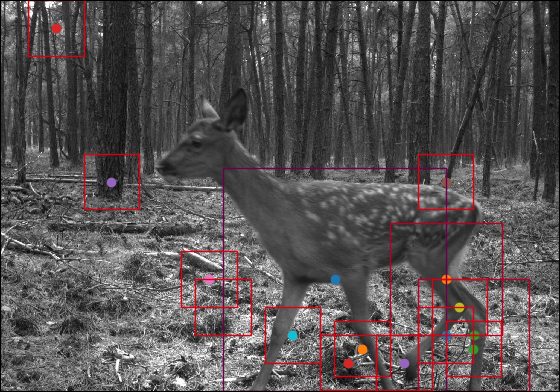
\includegraphics[width=8cm]{img/Segmentierung/localisation}
\end{tabular}
\captionof{figure}{ Lokalisierung mit Sliding-windows und PCA.}
\label{fig:loc}
\end{center}
